
\section{Architecture Integration}

\subsection{Model Support Matrix}

\begin{table}[H]
\centering
\small
\begin{tabular}{llllll}
\toprule
\textbf{Architecture} & \textbf{Attention} & \textbf{Nested?} & \textbf{RoPE?} & \textbf{GQA?} & \textbf{Path} \\
\midrule
DistilBERT & \texttt{MultiHeadSelfAttention} & No & No & No & Encoder \\
RoBERTa & \texttt{BertSelfAttention} & Yes & No & No & Encoder \\
GPT-2 & \texttt{GPT2Attention} & No & No & No & Decoder \\
Qwen3.5 & \texttt{Qwen3Attention} & No & Yes & Yes & Decoder \\
\bottomrule
\end{tabular}
\end{table}

\subsection{Weight Transfer Details}

\subsubsection{Detecting Nested Encoders}

The detection order matters. We check \texttt{has\_out} first:

\begin{lstlisting}
has\_out = any(hasattr(src, x) for x in ['dense', 'out\_proj', 'out\_lin', 'c\_proj', 'o\_proj'])
if cls\_name in ['BertSelfAttention', 'RobertaSelfAttention'] or (hasattr(src, 'query') and not has\_out):
    self.is\_nested\_encoder = True
if hasattr(src, 'self') and hasattr(src, 'output'):
    self.is\_nested\_encoder = True
\end{lstlisting}

\textbf{Key insight.} DistilBERT's \texttt{MultiHeadSelfAttention} ends with "SelfAttention" but has \texttt{out\_lin}, so \texttt{has\_out=True} and it is \textbf{not} classified as nested. This is correct.

\subsubsection{The RoPE Extraction Chain}

For Qwen:

\begin{lstlisting}
if hasattr(src, "rotary\_emb"):
    self.rotary\_emb = src.rotary\_emb
\end{lstlisting}

Then at forward time, we try three call signatures:

\begin{lstlisting}
try:
    cos, sin = rotary\_mod(Q, seq\_len=kv\_len)
except Exception:
    try:
        cos, sin = rotary\_mod(Q, pos\_ids)
    except Exception:
        try:
            cos, sin = rotary\_mod(Q)
        except Exception:
            cos, sin = None, None
\end{lstlisting}

\textbf{Fragile.} The triple-nested try/except works for common cases but fails 
silently for unusual RoPE implementations.

\subsection{The Two Attention Paths}

\subsubsection{Encoder Path (Bidirectional)}

\begin{lstlisting}
KV\_cos = torch.matmul(K\_cos.transpose(-2, -1), V)
KV\_sin = torch.matmul(K\_sin.transpose(-2, -1), V)
Z\_cos = K\_cos.sum(dim=2, keepdim=True)
Z\_sin = K\_sin.sum(dim=2, keepdim=True)

num = torch.matmul(Q\_cos, KV\_cos) + torch.matmul(Q\_sin, KV\_sin)
denom = torch.matmul(Q\_cos, Z\_cos.transpose(-2, -1)) + \
        torch.matmul(Q\_sin, Z\_sin.transpose(-2, -1)) + self.eps
context = num / denom.clamp(min=self.eps)
\end{lstlisting}

\textbf{4 matmuls, 2 sums.} Clean and fast.

\subsubsection{Decoder Path (Chunked)}

\begin{lstlisting}
chunk\_size = 32
if N \textless{}= chunk\_size:
    # Single chunk -- direct computation with causal mask
    ...
else:
    # Multiple chunks
    for c in range(num\_chunks):
        num\_inter = Q\_c @ S\_cos + Q\_sin @ S\_sin
        denom\_inter = Q\_c @ Z\_cos + Q\_sin @ Z\_sin
        # ... append, update state
\end{lstlisting}

\textbf{4 outer iterations for $L = 128$.} Each iteration ~5 kernel launches. 
Total ~20 extra kernel launches. Fast enough.

\subsection{Masking}

Masks are applied to \textbf{both K and V} (not just K):

\begin{lstlisting}
K = K * mask\_expanded
V = V * mask\_expanded
\end{lstlisting}

This is \textbf{critical} for the chunked scan -- otherwise padding tokens 
contribute to the state.

\subsection{Injection}

\textbf{Algorithm 2:} Inject CosformerAttention
\begin{lstlisting}
Input:  layer  , config, old\_attn
Output: new attention in  

1: new $\leftarrow$ CosformerAttention(config, old=old\_attn)
2: if copy\_weights fails: return None
3: if   has .attention.self:
4:      .attention.self $\leftarrow$ new; is\_nested $\leftarrow$ True
5: elif   has .attention:
6:      .attention $\leftarrow$ new
7: elif   has .self:  .self $\leftarrow$ new; is\_nested $\leftarrow$ True
8: elif   has .attn:  .attn $\leftarrow$ new
9: return new
\end{lstlisting}

\subsection{Common Pitfalls}

\subsubsection{RoPE Call Signature}

The triple-nested try/except for RoPE is fragile. If the RoPE implementation 
uses an unusual call signature, extraction fails silently.

\subsubsection{Nested Encoder Detection}

Getting \texttt{is\_nested\_encoder} wrong leads to double \texttt{out\_proj}.

\subsubsection{The `tau` Parameter is Unused}

\texttt{self.tau = nn.Parameter(torch.tensor(1.0), requires\_grad=False)} is 
declared but never used in \texttt{forward}. Dead code.

\subsubsection{Padding in the Chunked Scan}

Padding tokens must be masked in the state update. Otherwise, the state 
accumulates garbage.

\subsection{Registry}

\begin{lstlisting}
@ATTENTION\_REGISTRY.register("cosformer")
@ATTENTION\_REGISTRY.register("cosformer\_attention")
class CosformerAttention(BaseAttention):
    ...
\end{lstlisting}

\subsection{Integration with LoRA Recovery}

The standard pipeline applies:

\begin{enumerate}
\item Load pretrained model.
\item Inject Cosformer via \texttt{inject\_cosformer}.
\item Freeze base weights, keep LoRA trainable.
\item Run 50 recovery steps.
\item Evaluate.

\end{enumerate}
\subsection{Architecture-Specific Notes}

\subsubsection{DistilBERT}

\begin{itemize}
\item \textbf{Path:} Encoder
\item \textbf{Nested:} No
\item \textbf{RoPE:} No

\end{itemize}
\subsubsection{RoBERTa}

\begin{itemize}
\item \textbf{Path:} Encoder
\item \textbf{Nested:} Yes (output projection via outer \texttt{output.dense})
\item \textbf{RoPE:} No
\item \textbf{Complication:} RoBERTa's \texttt{BertAttention} wraps \texttt{self} and \texttt{output}. We
  replace \texttt{self}. The outer \texttt{output.dense} applies the projection.

\end{itemize}
\subsubsection{GPT-2}

\begin{itemize}
\item \textbf{Path:} Decoder
\item \textbf{Nested:} No
\item \textbf{RoPE:} No
\item \textbf{Complication:} GPT-2 uses Conv1D weight layout (transposed).

\end{itemize}
\subsubsection{Qwen3.5}

\begin{itemize}
\item \textbf{Path:} Decoder
\item \textbf{Nested:} No
\item \textbf{RoPE:} Yes
\item \textbf{GQA:} Yes
\item \textbf{Complication:} RoPE extraction from HuggingFace API is fragile.
\end{itemize}
\begin{lstlisting}

---
\end{lstlisting}

\begin{figure}[H]
\centering
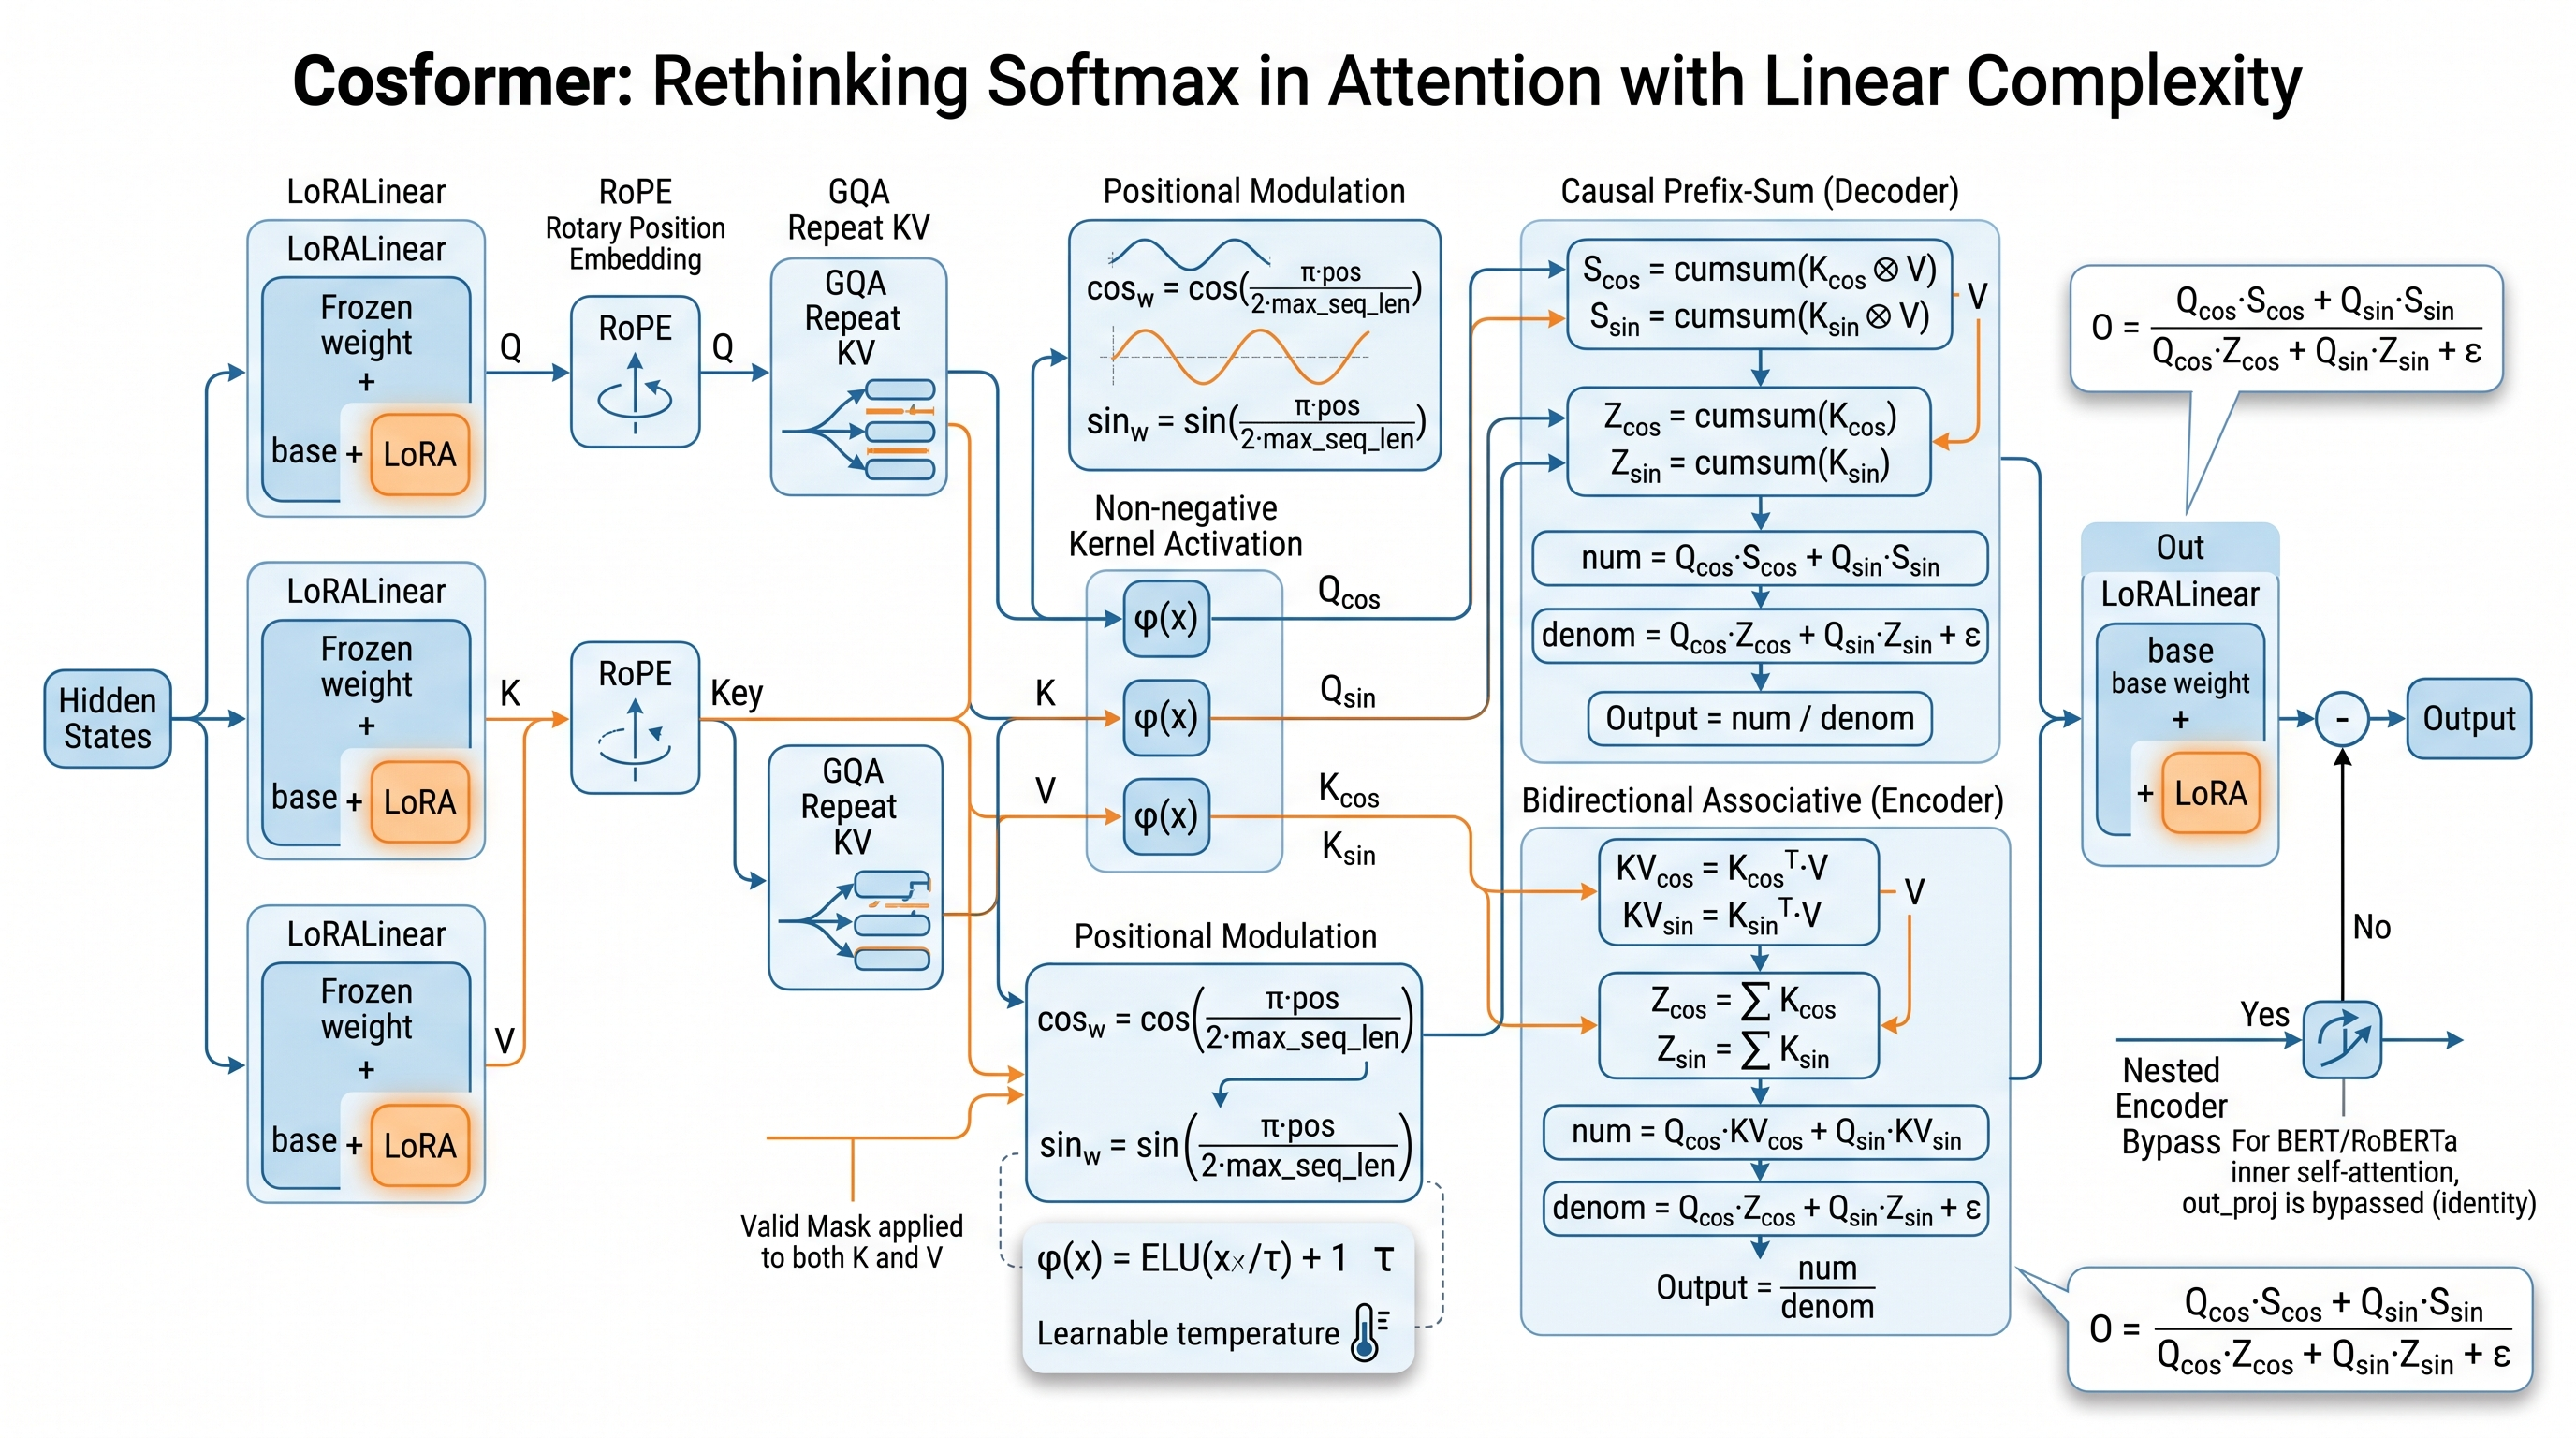
\includegraphics[width=\linewidth]{figures/architecture.jpeg}
\caption{High-level architectural diagram of cosformer.}
\label{fig:arch\_cosformer}
\end{figure}

